\documentclass[tikz]{standalone}
\usetikzlibrary{positioning, arrows.meta}

\begin{document}
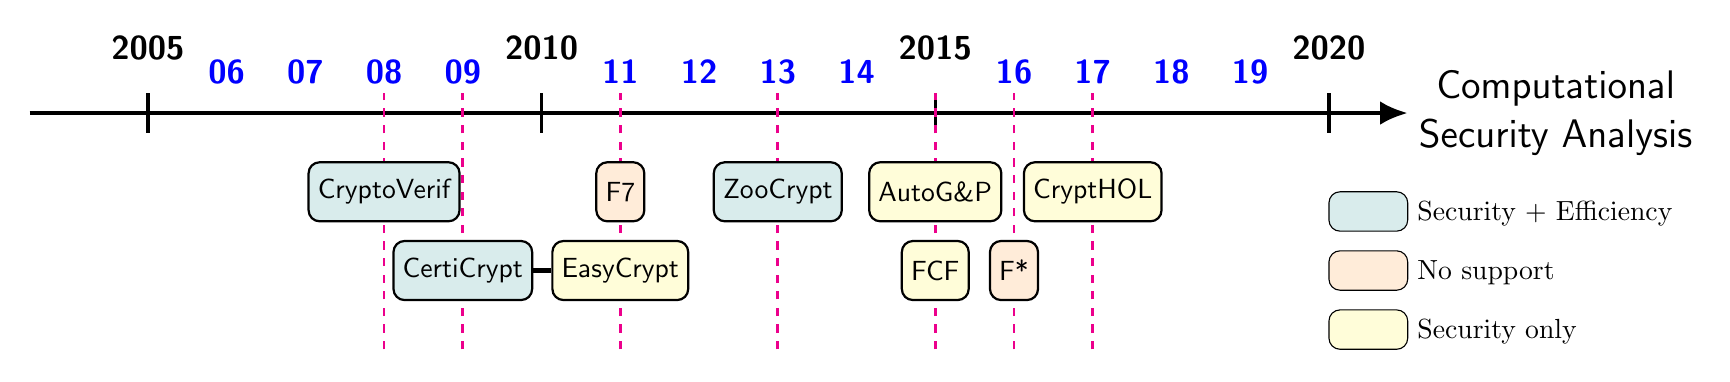
\begin{tikzpicture}[
	node distance=1cm and 2cm,
	event/.style={
		rectangle,
		rounded corners=4pt,
		draw=black,
		thick,
		fill=blue!20,
		text width=6cm,
		align=center,
		font=\sffamily,
		minimum height=1cm
	},
	event2/.style={
		rectangle,
		rounded corners=4pt,
		draw=black,
		thick,
		fill=orange!20,
		text width=8cm,
		align=center,
		font=\sffamily,
		minimum height=1cm
	},
	event3/.style={
		rectangle,
		rounded corners=4pt,
		draw=black,
		thick,
		fill=teal!20,
		text width=8cm,
		align=center,
		font=\sffamily,
		minimum height=1cm
	},
	year/.style={
		font=\sffamily\bfseries\large,
		anchor=south
	},
	node/.style={
		rectangle,
		rounded corners=4pt,
		draw=black,
		thick,
		fill=white,
		align=center,
		font=\sffamily,
		minimum height=.75cm
	},
	unbounded/.style={
		rectangle,
		rounded corners=4pt,
		draw=black,
		thick,
		fill=teal!15,
		align=center,
		font=\sffamily,
		minimum height=.75cm
	},
	bounded/.style={
		rectangle,
		rounded corners=4pt,
		draw=black,
		thick,
		fill=orange!15,
		align=center,
		font=\sffamily,
		minimum height=.75cm
	},
	equiv/.style={
		rectangle,
		rounded corners=4pt,
		draw=black,
		thick,
		fill=yellow!15,
		align=center,
		font=\sffamily,
		minimum height=.75cm
	}
	]
	\draw[line width=1.5pt, -{Latex[length=3.5mm, width=3mm]}] (-1.5,0) -- (16,0) node[right, font=\Large\sffamily, align=center] {Computational\\ Security Analysis};
	
	\draw[fill=teal!15, rounded corners=4pt] (15,-1.5) rectangle (16,-1) node[below right] {Security + Efficiency};
	\draw[fill=orange!15, rounded corners=4pt] (15,-2.25) rectangle (16,-1.75) node[below right] {No support};
	\draw[fill=yellow!15, rounded corners=4pt] (15,-3) rectangle (16,-2.5) node[below right] {Security only};
	
	\foreach \x/\yeartext in {0/2005, 5/2010, 10/2015, 15/2020}{
		\draw[line width=1.2pt] (\x, -0.25) -- (\x, 0.25);
		\node[year, above=0.3cm of {\x,0.25}] {\yeartext};
	}
	
	% Position the event nodes relative to coordinates on the timeline
%	\draw[red, fill=red] (8,0) circle (2.5pt) node[below=.25cm] {NOW};
%	\node[year, above=0cm of {-1,0.25}, blue] {04};
	\node[year, above=0cm of {1,0.25}, blue] {06};
	\node[year, above=0cm of {2,0.25}, blue] {07};
	\node[year, above=0cm of {3,0.25}, blue] {08};
	\node[year, above=0cm of {4,0.25}, blue] {09};
	\node[year, above=0cm of {6,0.25}, blue] {11};
	\node[year, above=0cm of {7,0.25}, blue] {12};
	\node[year, above=0cm of {8,0.25}, blue] {13};
	\node[year, above=0cm of {9,0.25}, blue] {14};
	\node[year, above=0cm of {11,0.25}, blue] {16};
	\node[year, above=0cm of {12,0.25}, blue] {17};
	\node[year, above=0cm of {13,0.25}, blue] {18};
	\node[year, above=0cm of {14,0.25}, blue] {19};
	
	\foreach \x in {3,4,6,8,10,11,12}{
		\draw[line width=1pt, dashed, magenta] (\x, -3) -- (\x, 0.25);
	}

	\node[bounded] (F7) at (6,-1) {F7}; % 11
	\node[equiv] (AutoGP) at (10,-1) {AutoG\&P}; % 15
	\node[unbounded] (CertiCrypt) at (4,-2) {CertiCrypt}; % 9
	\node[equiv] (CryptHOL) at (12,-1) {CryptHOL}; % 17
	\node[unbounded] (CryptoVerif) at (3,-1) {CryptoVerif}; % 8
	\node[equiv] (EasyCrypt) at (6,-2) {EasyCrypt}; % 11
	\node[bounded] (F) at (11,-2) {F*}; % 16
	\node[equiv] (FCF) at (10,-2) {FCF}; % 15
	\node[unbounded] (ZooCrypt) at (8,-1) {ZooCrypt}; % 13
	
	\draw[line width=1.5pt] (CertiCrypt.east) to (EasyCrypt.west);
%	\draw[line width=1.5pt] (Tamarin.east) -| (SAPIC.north);
%	\draw[line width=1.5pt] (fs2pv.east) -| (StatVerif.west);
%	\draw[line width=1.5pt] (StatVerif.east) -| (ProVerif.west);
%	\draw[line width=1.5pt] (ProVerif.east) -| (GSVerif.west);
%	\draw[line width=1.5pt] (GSVerif.east) -| (ProVerif-ATP.north);
\end{tikzpicture}
\end{document}